\documentclass[11pt]{article}

\usepackage{mathtools}
\usepackage{float}
\usepackage{amssymb}
\usepackage{amsmath}
\usepackage{amsthm}
\usepackage{hyperref}
\usepackage{microtype}
\usepackage{graphicx}
\usepackage{blkarray}
\usepackage{pgfplots}
\pgfplotsset{compat=1.15}
\usepackage{mathrsfs}
\usetikzlibrary{arrows}
\graphicspath{ {./img/} }

\setlength{\parindent}{0cm}
\let\emptyset\varnothing

\title{\textbf{CSCI/MATH 2113 Discrete Structures} \\ Chapter 12 Trees}
\author{Alyssa Motas}

\begin{document}

    \maketitle

    \pagebreak

    \tableofcontents

    \pagebreak

    \section{12.1 Definitions, Properties, and Examples}

    \subsection{Tree}

    Let \(G = (V,E)\) be a loop-free undirected graph. The graph $G$ is called a \emph{tree} if $G$ is connected and contains no cycles.

    \emph{Remark:} Often simply a connected cycle-free graph.

    \subsubsection{Example}

    \begin{figure}[H]
        \centering
        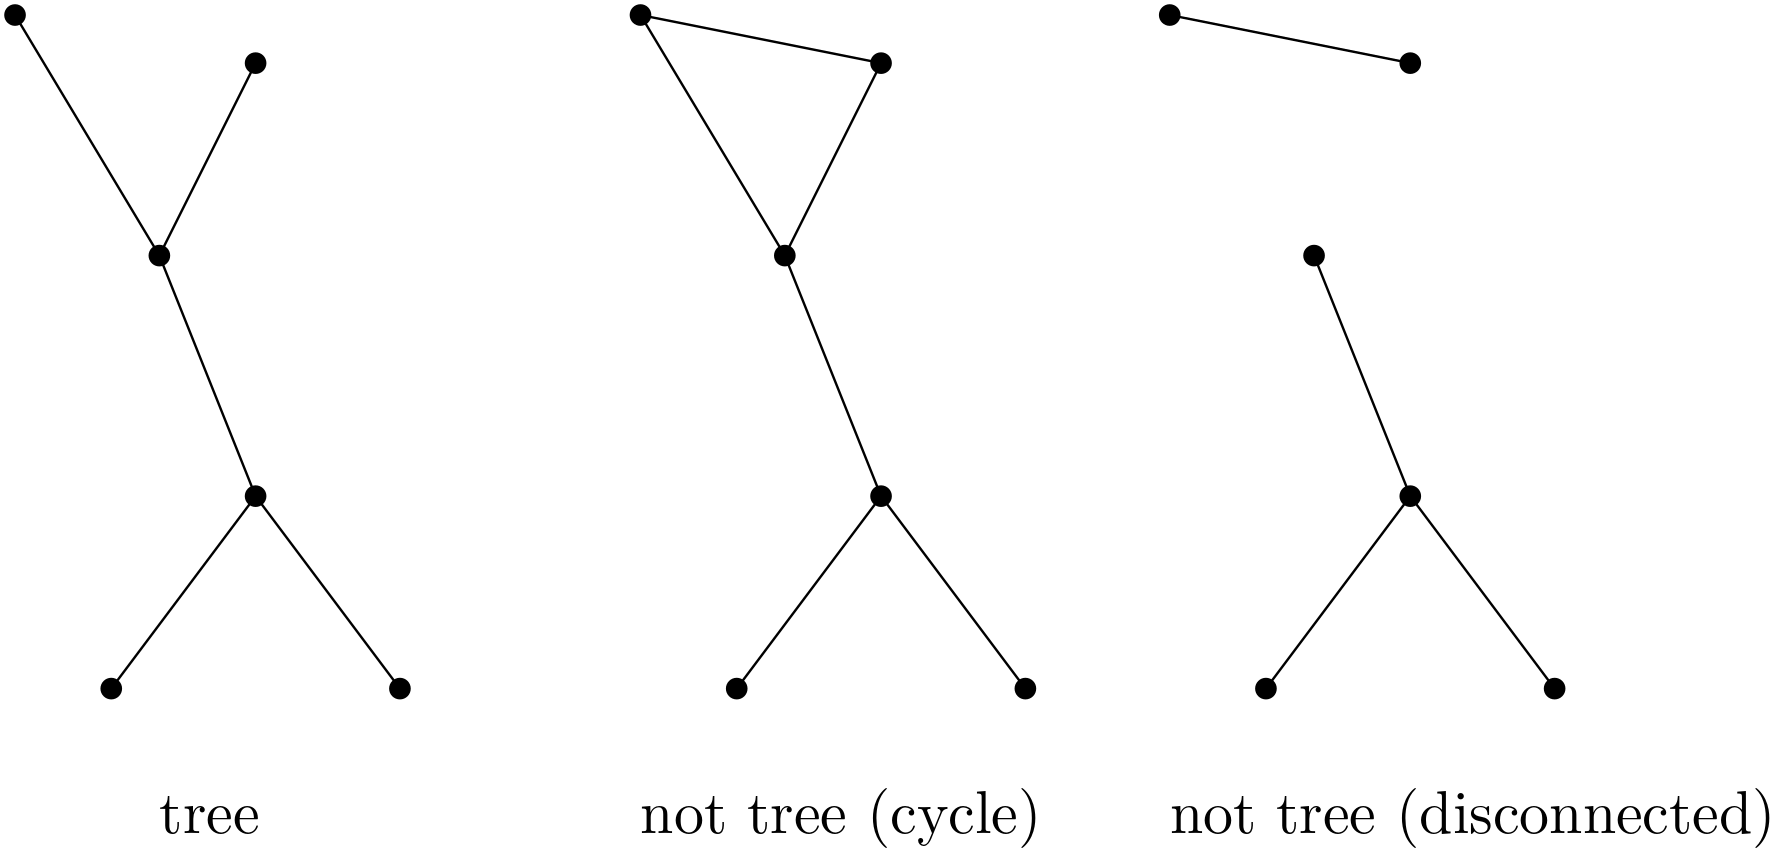
\includegraphics[scale=0.2]{trees.png}
    \end{figure}

    A collection of disconnected trees is a \emph{forest}. 

    \subsection{Spanning tree}

    A \emph{spanning tree} for a graph $G$ is a spanning subgraph of $G$ that is a tree.

    \subsection{Unique path between two distinct vertices in a tree}

    If \(a,b\) are distinct vertices in a tree \(T = (V,E)\), then there is a unique path that connects these vertices.
    \begin{proof}
        There is a path since $T$ is connected. There is at most one path since otherwise $T$ would contain a cycle.
    \end{proof}

    \subsection{Condition of a connected graph}

    If \(G = (V,E)\) is an undirected graph, then $G$ is connected if and only if $G$ has a spanning tree.
    \begin{proof}
        \(\Leftarrow\) If $G$ has a spanning tree, then there is a path between any two vertices of $G$ along a subgraph of $G$ (and thus in $G$).

        \(\Rightarrow\) Assume that $G$ is connected. Consider the subgraph containing no loops. If $G$ (without loops) is a tree then we are done. Ohterwise, $G$ has a cycle and we can consider an edge \(e_1\) in this cycle. Then consider the subgraph \(G_1 = G - e_1\). If \(G_1\) is a tree then we are done. Otherwise, we repeat this process.
    \end{proof}

    \subsection{Non-isomorphic trees}

    Three trees with 5 vertices:
    \begin{figure}[H]
        \centering
        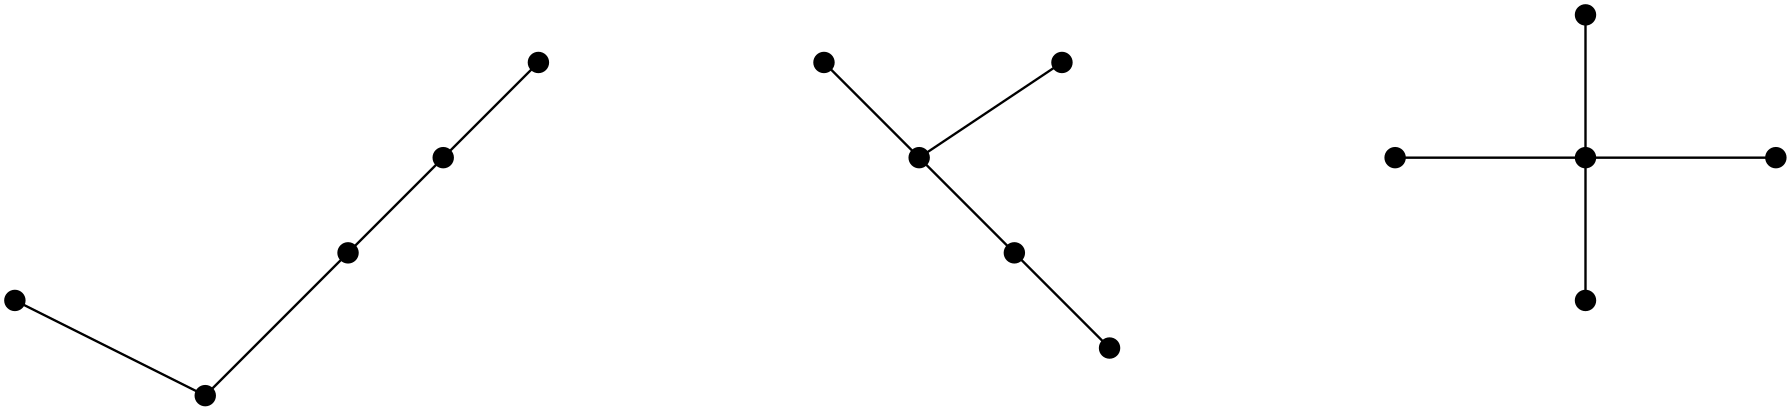
\includegraphics[scale=0.2]{noniso.png}
    \end{figure}

    None of these graphs are isomorphic (e.g., the third graph has a vertex of degree 4 whereas none of the others do.)

    \pagebreak
    
    \subsection{Number of edges in a tree}

    In every tree \(T = (V,E)\), \(|V| = |E| + 1\).
    \begin{proof}
        By induction on \(|E|\): If \(|E| = 0\), then $T$ has one vertex and so \(|V| = 1\), and the equation holds. If \(|E| = 1\), then $T$ has two vertices, so \(|V| = 2\). If \(|E| = 2\), then $T$ has three vertices so \(|V| = 3\). If \(|E| = k+1\) then $T$ is of the form
        \begin{figure}[H]
            \centering
            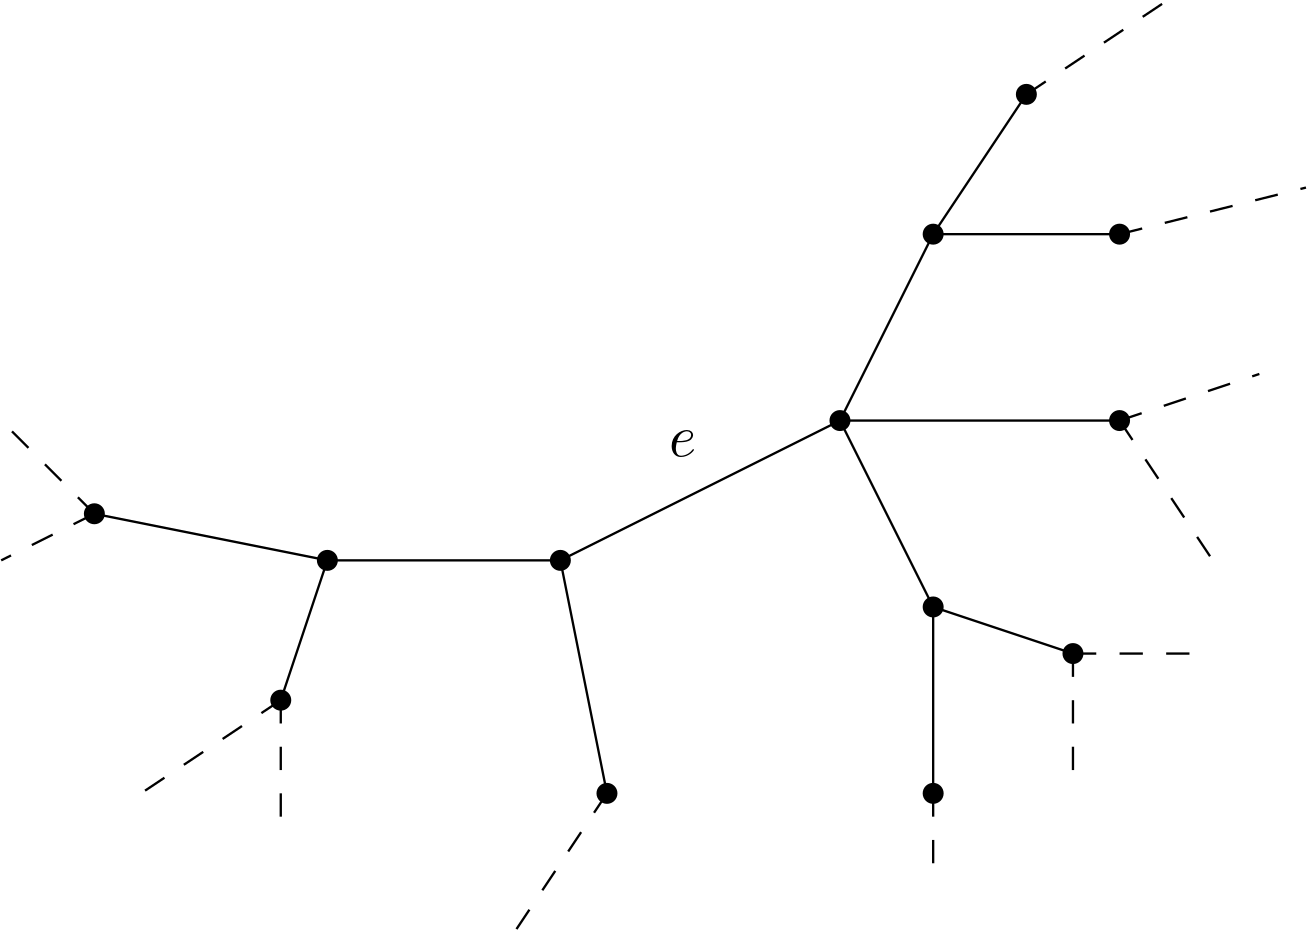
\includegraphics[scale=0.1]{e.png}
        \end{figure}
        Removing $e$ from $T$ gives us a forest 
        \begin{figure}[H]
            \centering
            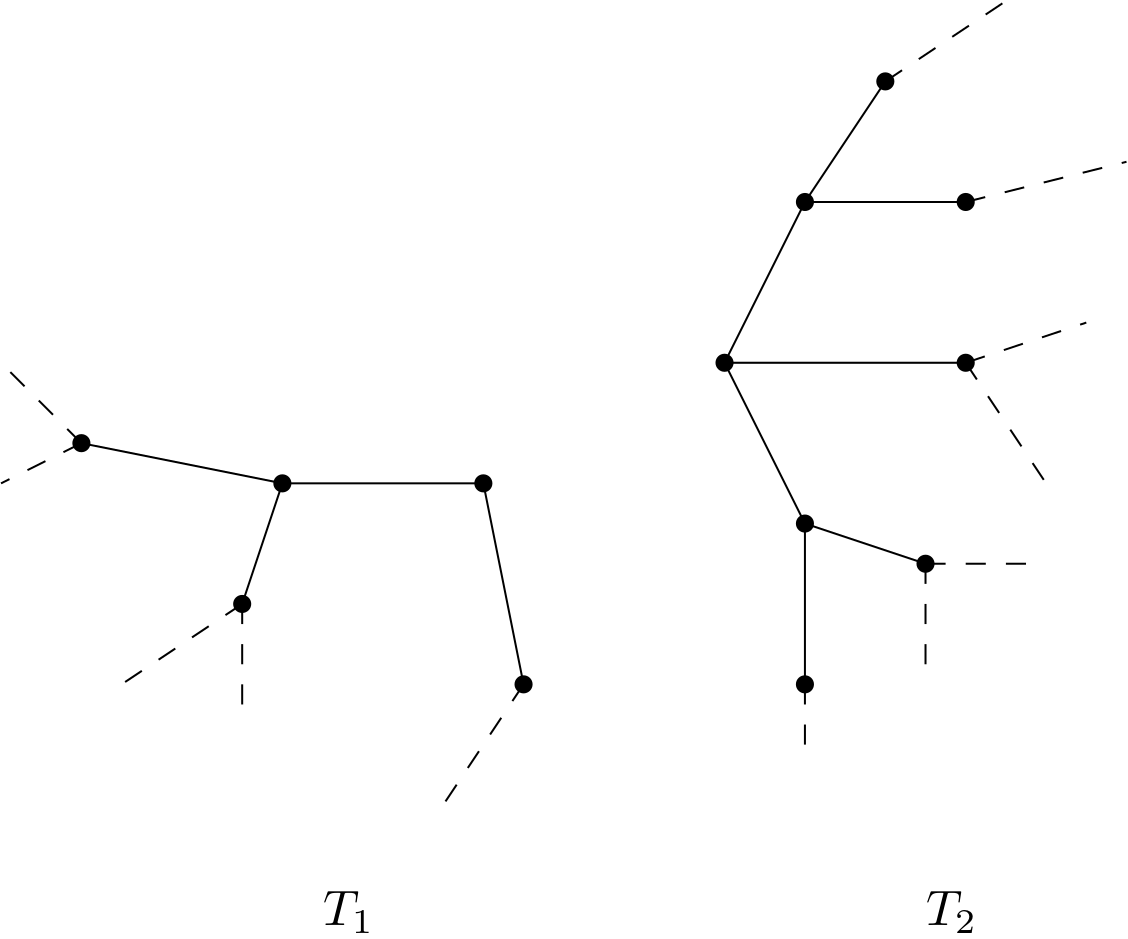
\includegraphics[scale=0.1]{forest.png}
        \end{figure}
        Then \(T_1\) and \(T_2\) are smaller trees, i.e. \(T_1 = (V_1, E_1)\) and \(T_2 = (V_2, E_2)\). And \[0 \leq |E_1| \leq k \quad \text{and} \quad 0 \leq |E_2| \leq k.\] Hence \[|V_1| = |E_1| + 1 \quad \text{and} \quad |V_2| = |E_2| + 1.\] Thus \[|V| = |V_1| + |V_2| = |E_1| + 1 + |E_2| + 1 = |E| + 1.\]
    \end{proof}

    \subsection{Pendant vertices}

    If \(T = (V,E)\) is a tree with \(|V| \geq 2\) then $T$ has at least 2 pendant vertices.
    \begin{proof}
        We have \(|E| = |V| - 1\) and \[2|E| = \sum_{v \in V} \deg(v).\] Hence \(2(|V| - 1) = \sum_{v \in V} \deg (v)\). Let $k$ be the number of pendant vertices. Then
        \begin{align*}
            2(|V| - 1) &= \sum_{v \in V} \deg(v) \\
                       &\geq k + 2 (|V| - k)
        \end{align*}
        since the graph is connected, there are no vertices of degree 0. Then \(2(|V| - 1) \geq k+2(|V| - k)\) implies \(k \geq 2\). 
    \end{proof}

    \subsection{Properties of a tree}

    The following statements are equivalent for a loop-free undirected graph \(G = (V,E)\).
    \begin{enumerate}
        \item $G$ is a tree.
        \item $G$ is connected and removing an edge leaves a forest of two trees.
        \item $G$ contains no cycles and \(|V| = |E| + 1\). 
        \item $G$ is connected and \(|V| = |E| + 1\).
        \item $G$ contains no cycles and if \(a,b \in V\) with \(\{a,b\} \notin E\) then adding \(\{a,b\}\) to $E$ yields exactly one cycle. 
    \end{enumerate}

    \section{12.2 Rooted Trees}

    \subsection{In- and out-degree}

    If \(G = (V,E)\) is a directed graph and \(v \in V\) then \(in(v)\), the \emph{in-degree} of $v$, is the number of edges ending at $v$. Similarly, \(out(v)\), the \emph{out-degree} of $v$, is the number of edges leaving $v$. 

    \subsection{Underlying undirected graph}

    If \(G = (V,E)\) is a directed graph then the \emph{underlying undirected graph} is the undirected graph obtained by forgetting the orientation of the edges. 

    \subsubsection{Example}

    In 
    \begin{figure}[H]
        \centering
        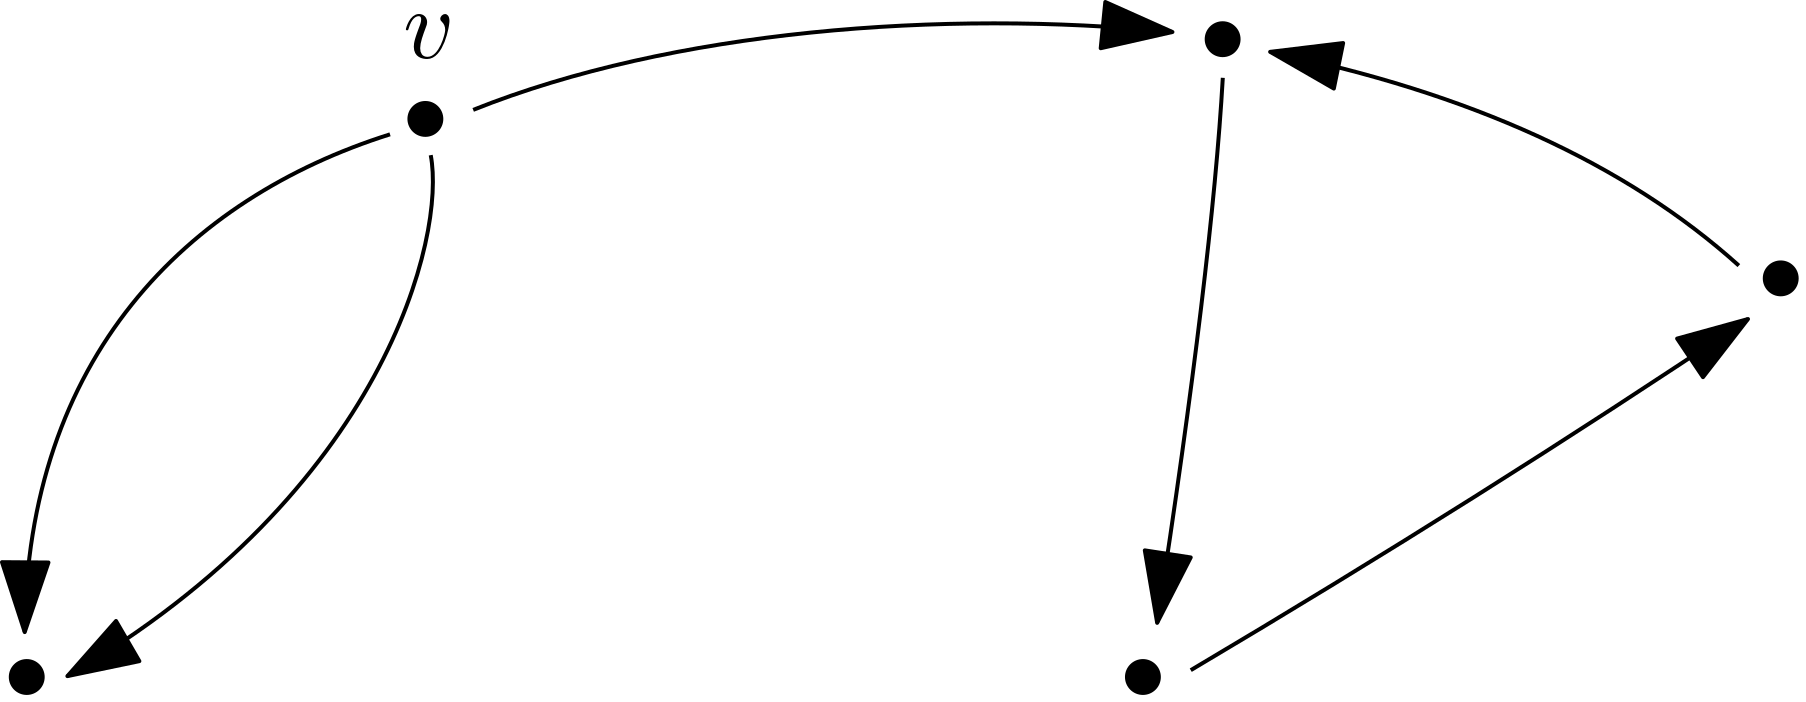
\includegraphics[scale=0.1]{inout.png}
    \end{figure}
    we have \(in(v) = 0\) and \(out(v) = 3\). And the underlying undirected graph is
    \begin{figure}[H]
        \centering
        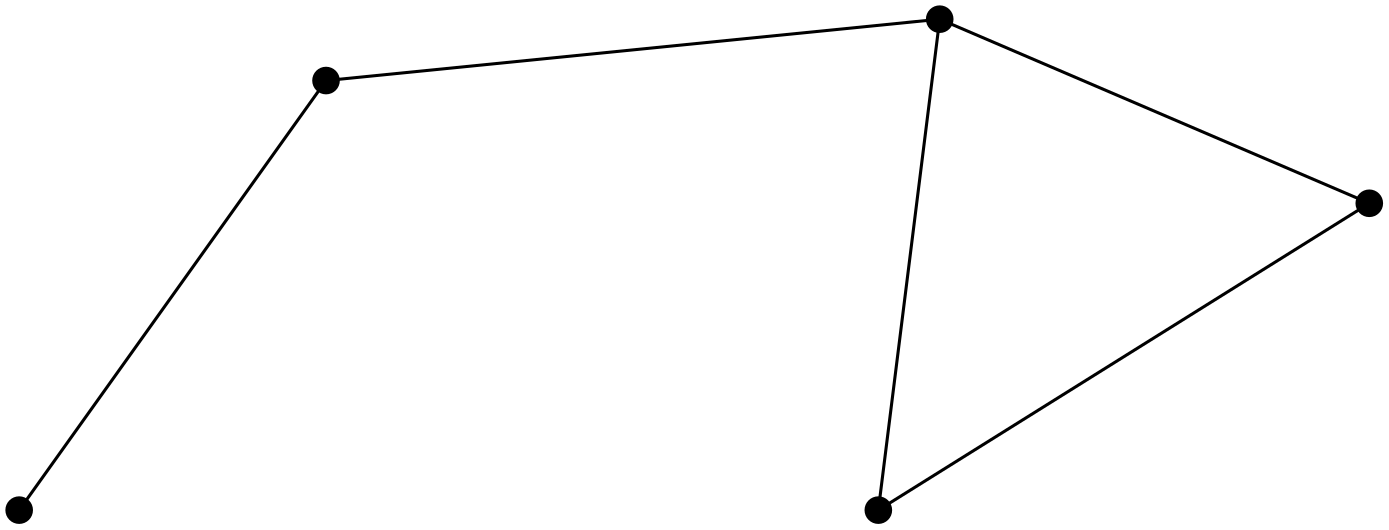
\includegraphics[scale=0.1]{underlying.png}
    \end{figure}

    \subsection{Directed tree and rooted tree}

    A directed graph $G$ is a \emph{directed tree} if the underlying graph is a tree. A directed tree $G$ is \emph{rooted} if there is a unique vertex $r$ with \(in(r) = 0\) and, for all other vertices $v$, \(in(v) = 1\). In this case, $r$ is the \emph{root}. 

    \vspace{1em}

    \emph{Remark:} The root is the only vertex without an incoming edge. 

    \subsection{Terminology:}
    \begin{itemize}
        \item the \emph{root} has in-degree 0
        \item the \emph{leaves} have out-degree 0
        \item the nodes that are neither root nor leaf are called \emph{branch nodes}
        \item the length of the path from the root to a node is the \emph{level} of that node
        \item If there is a directed path from a node $n$ to a node $m$, we say that $n$ is an \emph{ancestor} of $m$ and that $m$ is a \emph{descendant} of $n$
        \item If the length of the path is 1 then $n$ is a \emph{parent} of $m$ and $m$ is a \emph{child} of $n$. 
    \end{itemize}

    \begin{figure}[H]
        \centering
        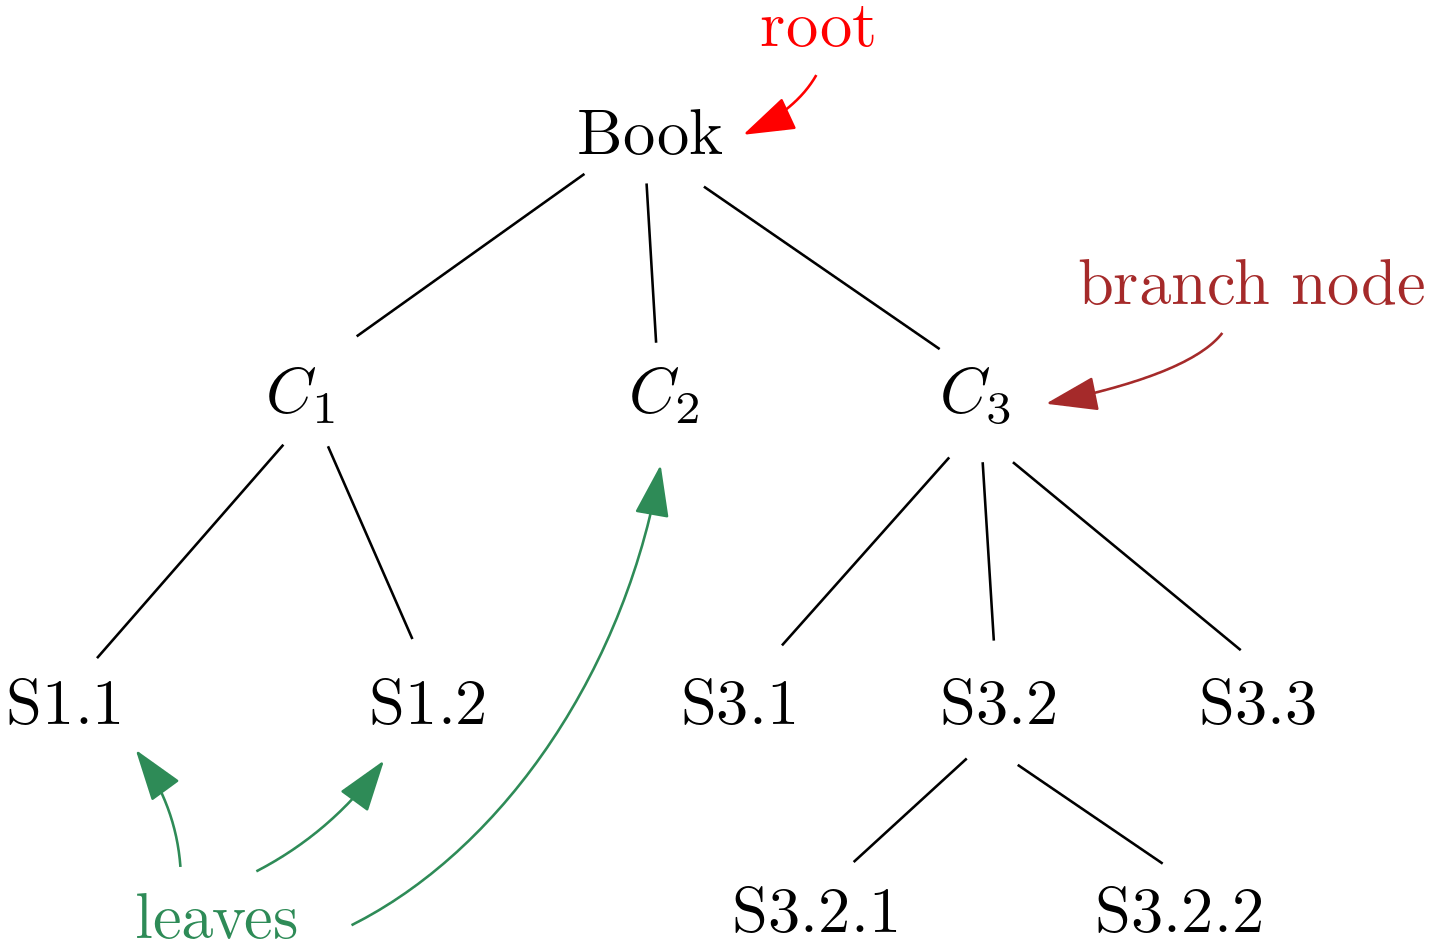
\includegraphics[scale=0.2]{root.png}
    \end{figure}

    \subsection{Lexicographic order}

    Consider the rooted tree
    \begin{figure}[H]
        \centering
        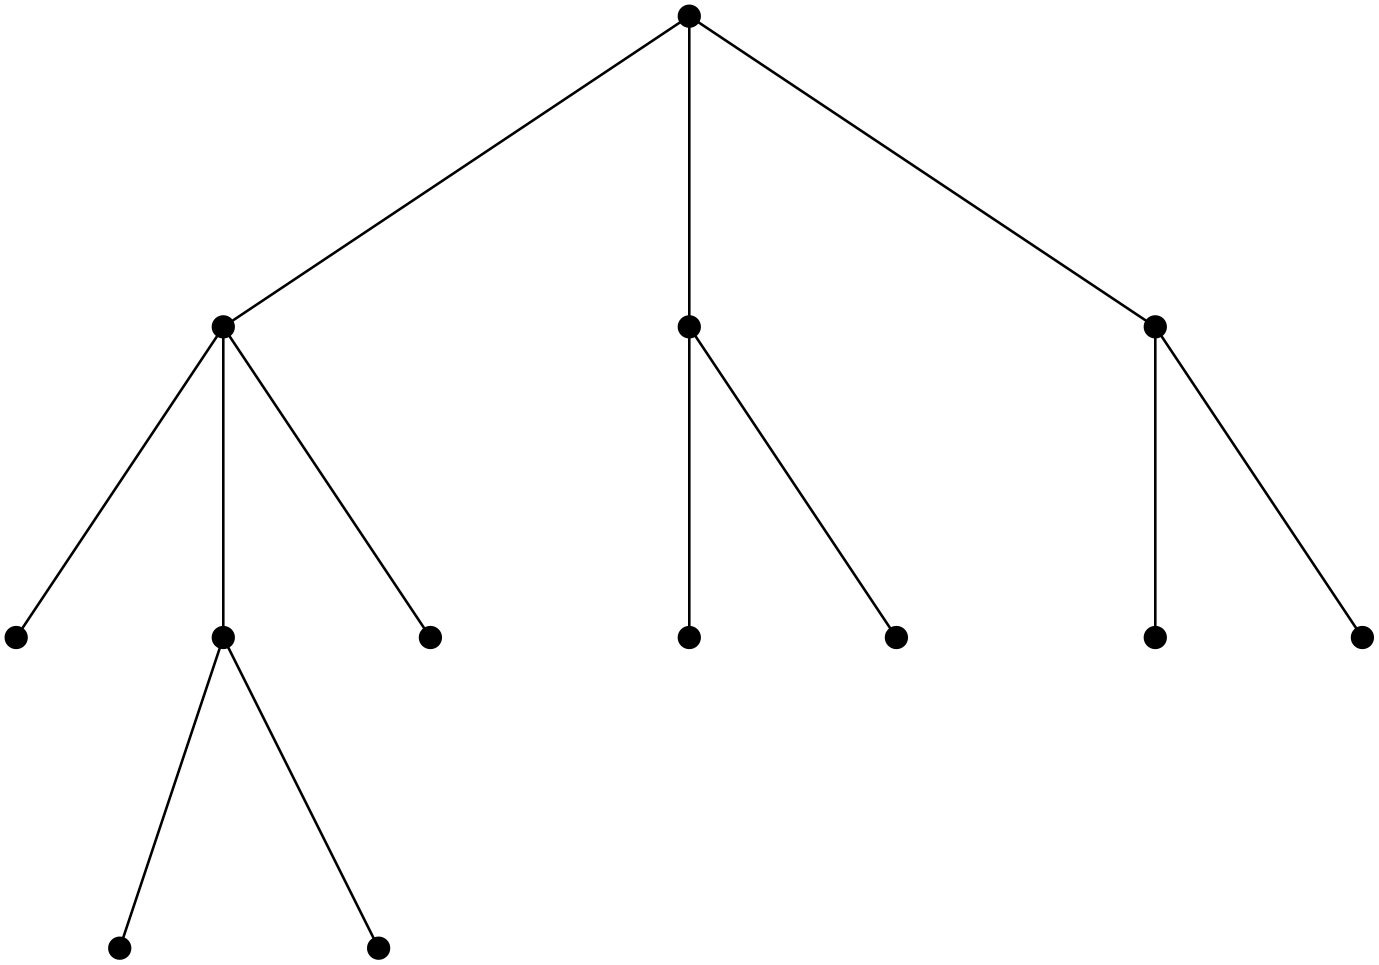
\includegraphics[scale=0.2]{lexi.png}
    \end{figure}
    Here, we consider the nodes at a given level as ordered from left to right. And labelling the nodes as above yields a total order on the set of vertices called the \emph{lexicographic order}.

    \subsection{Binary rooted tree}

    A rooted tree is a \emph{binary} rooted tree if the out-degree of a vertex is 0,1, or 2.

    \subsubsection{Example}

    Consider a binary operation such as \(+\) (addition). Then expressions involving \(+\) can be represented as binary trees. 
    \begin{figure}[H]
        \centering
        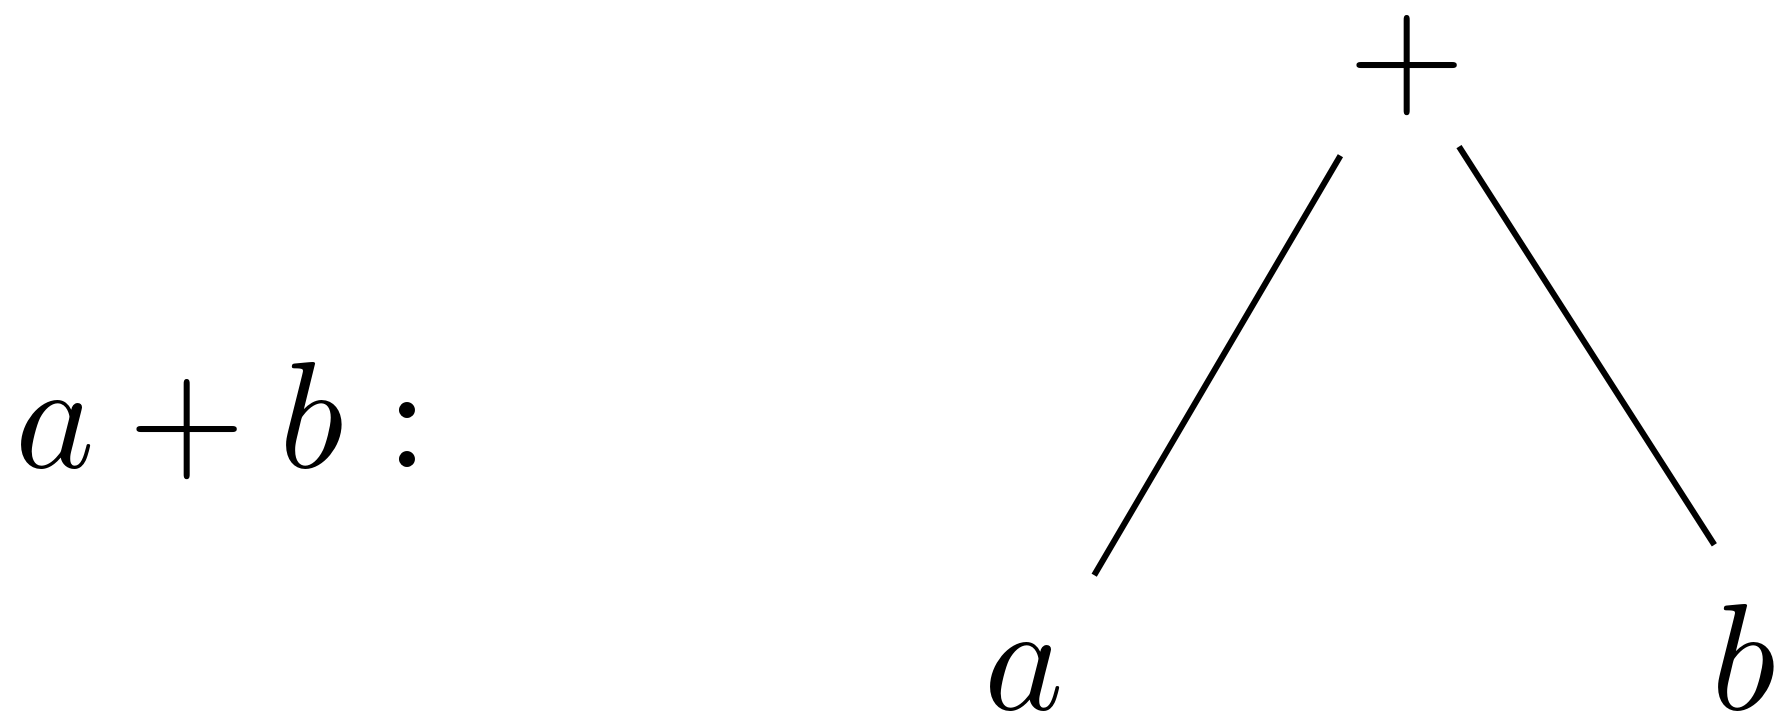
\includegraphics[scale=0.1]{ab.png}
    \end{figure}

    Similarly, an expression such as \[((7-a)/5)\times((a+b)^3)\] can be represented as 
    \begin{figure}[H]
        \centering
        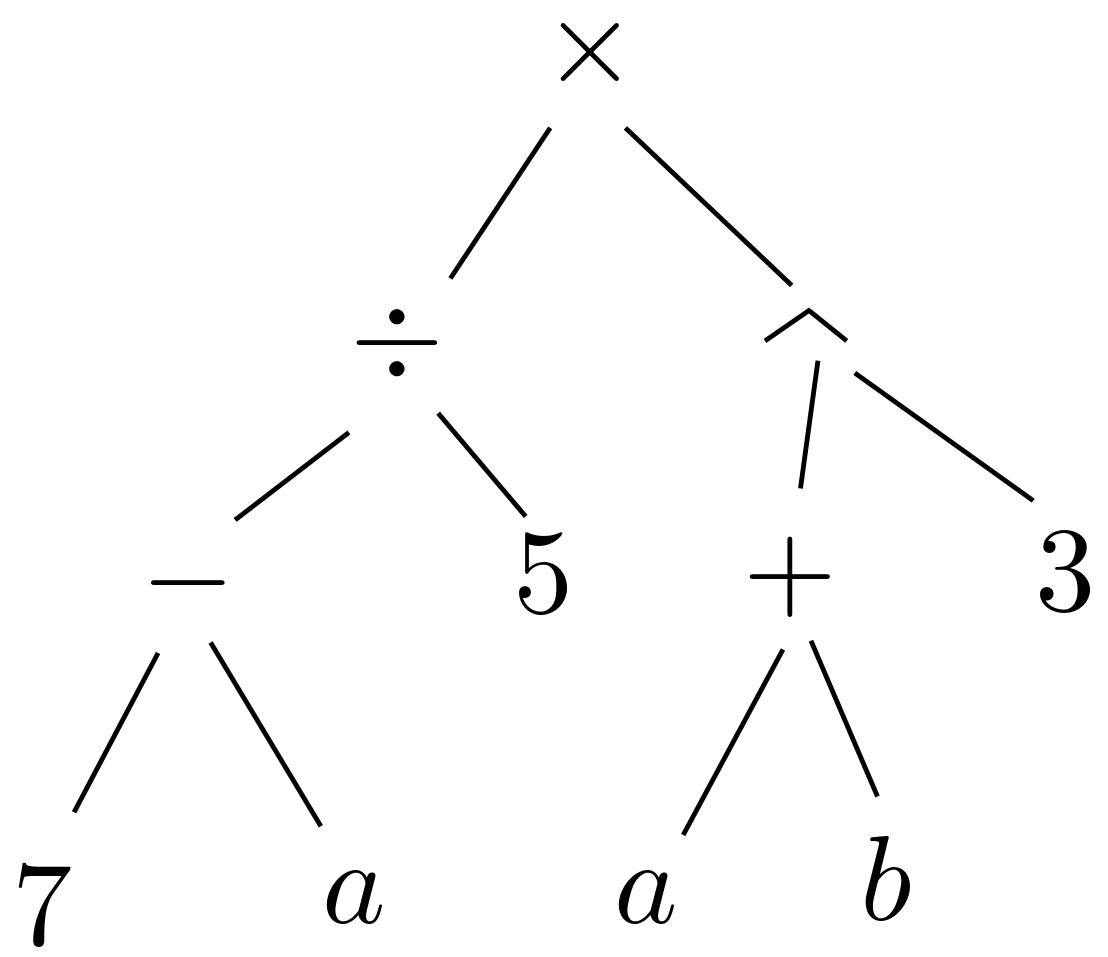
\includegraphics[scale=0.1]{finalex.png}
    \end{figure}

\end{document}